\section{Case} \setAuthor{Richard Krammer}
    There were cases designed for every module to protect the electronics inside and
    give the modules a finished look. The cases were only designed for the final versions of
    the modules. It was designed in Fusion 360 and manifactured with a FDM 3D printer. 

    \FloatBarrier
    \subsection{Basic}

        This case consists of two parts, the top and the bottom. The top part has 
        a cutout for the temperature sensor, LEDs the spare header and the 
        serial interface.

        \begin{figure}[htbp]
            \centering
            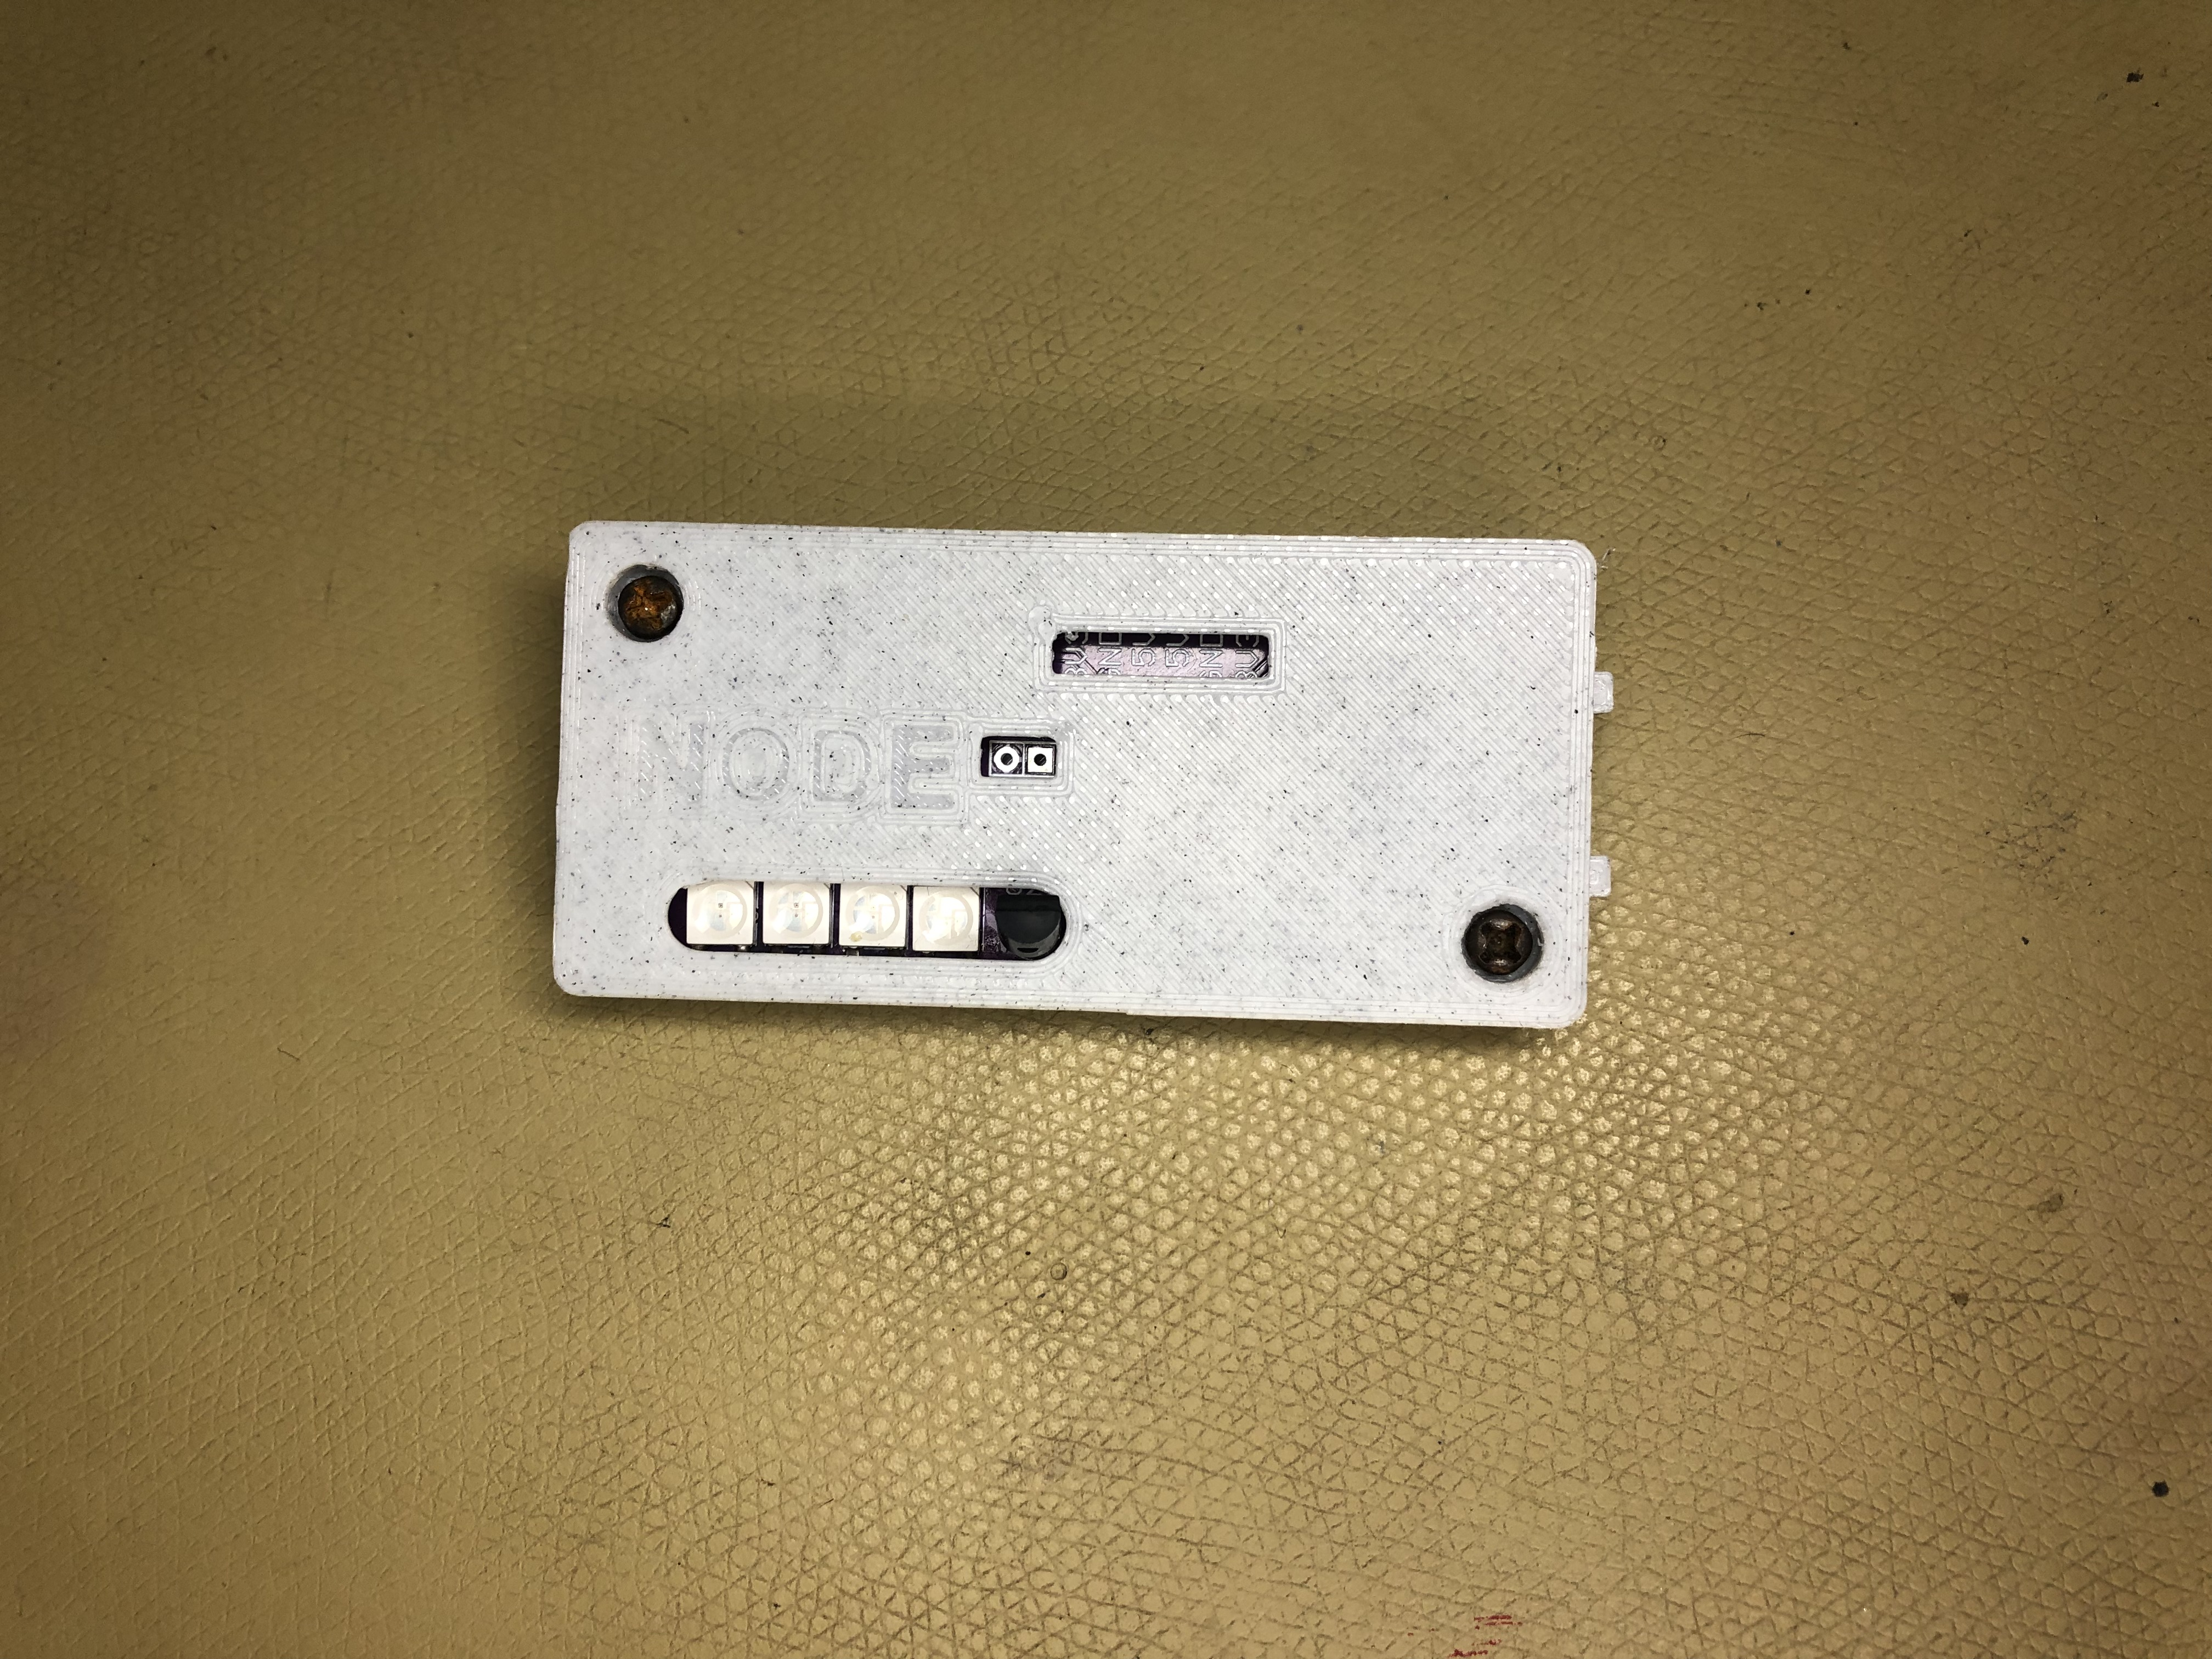
\includegraphics[width=0.8\textwidth]{assets/case/Node-Top2.JPG}
            \caption{Top view.}
        \end{figure}
        \needspace{5\baselineskip}
        The bottom part has a cutout for the module connector.
        \begin{figure}[htbp]
            \centering
            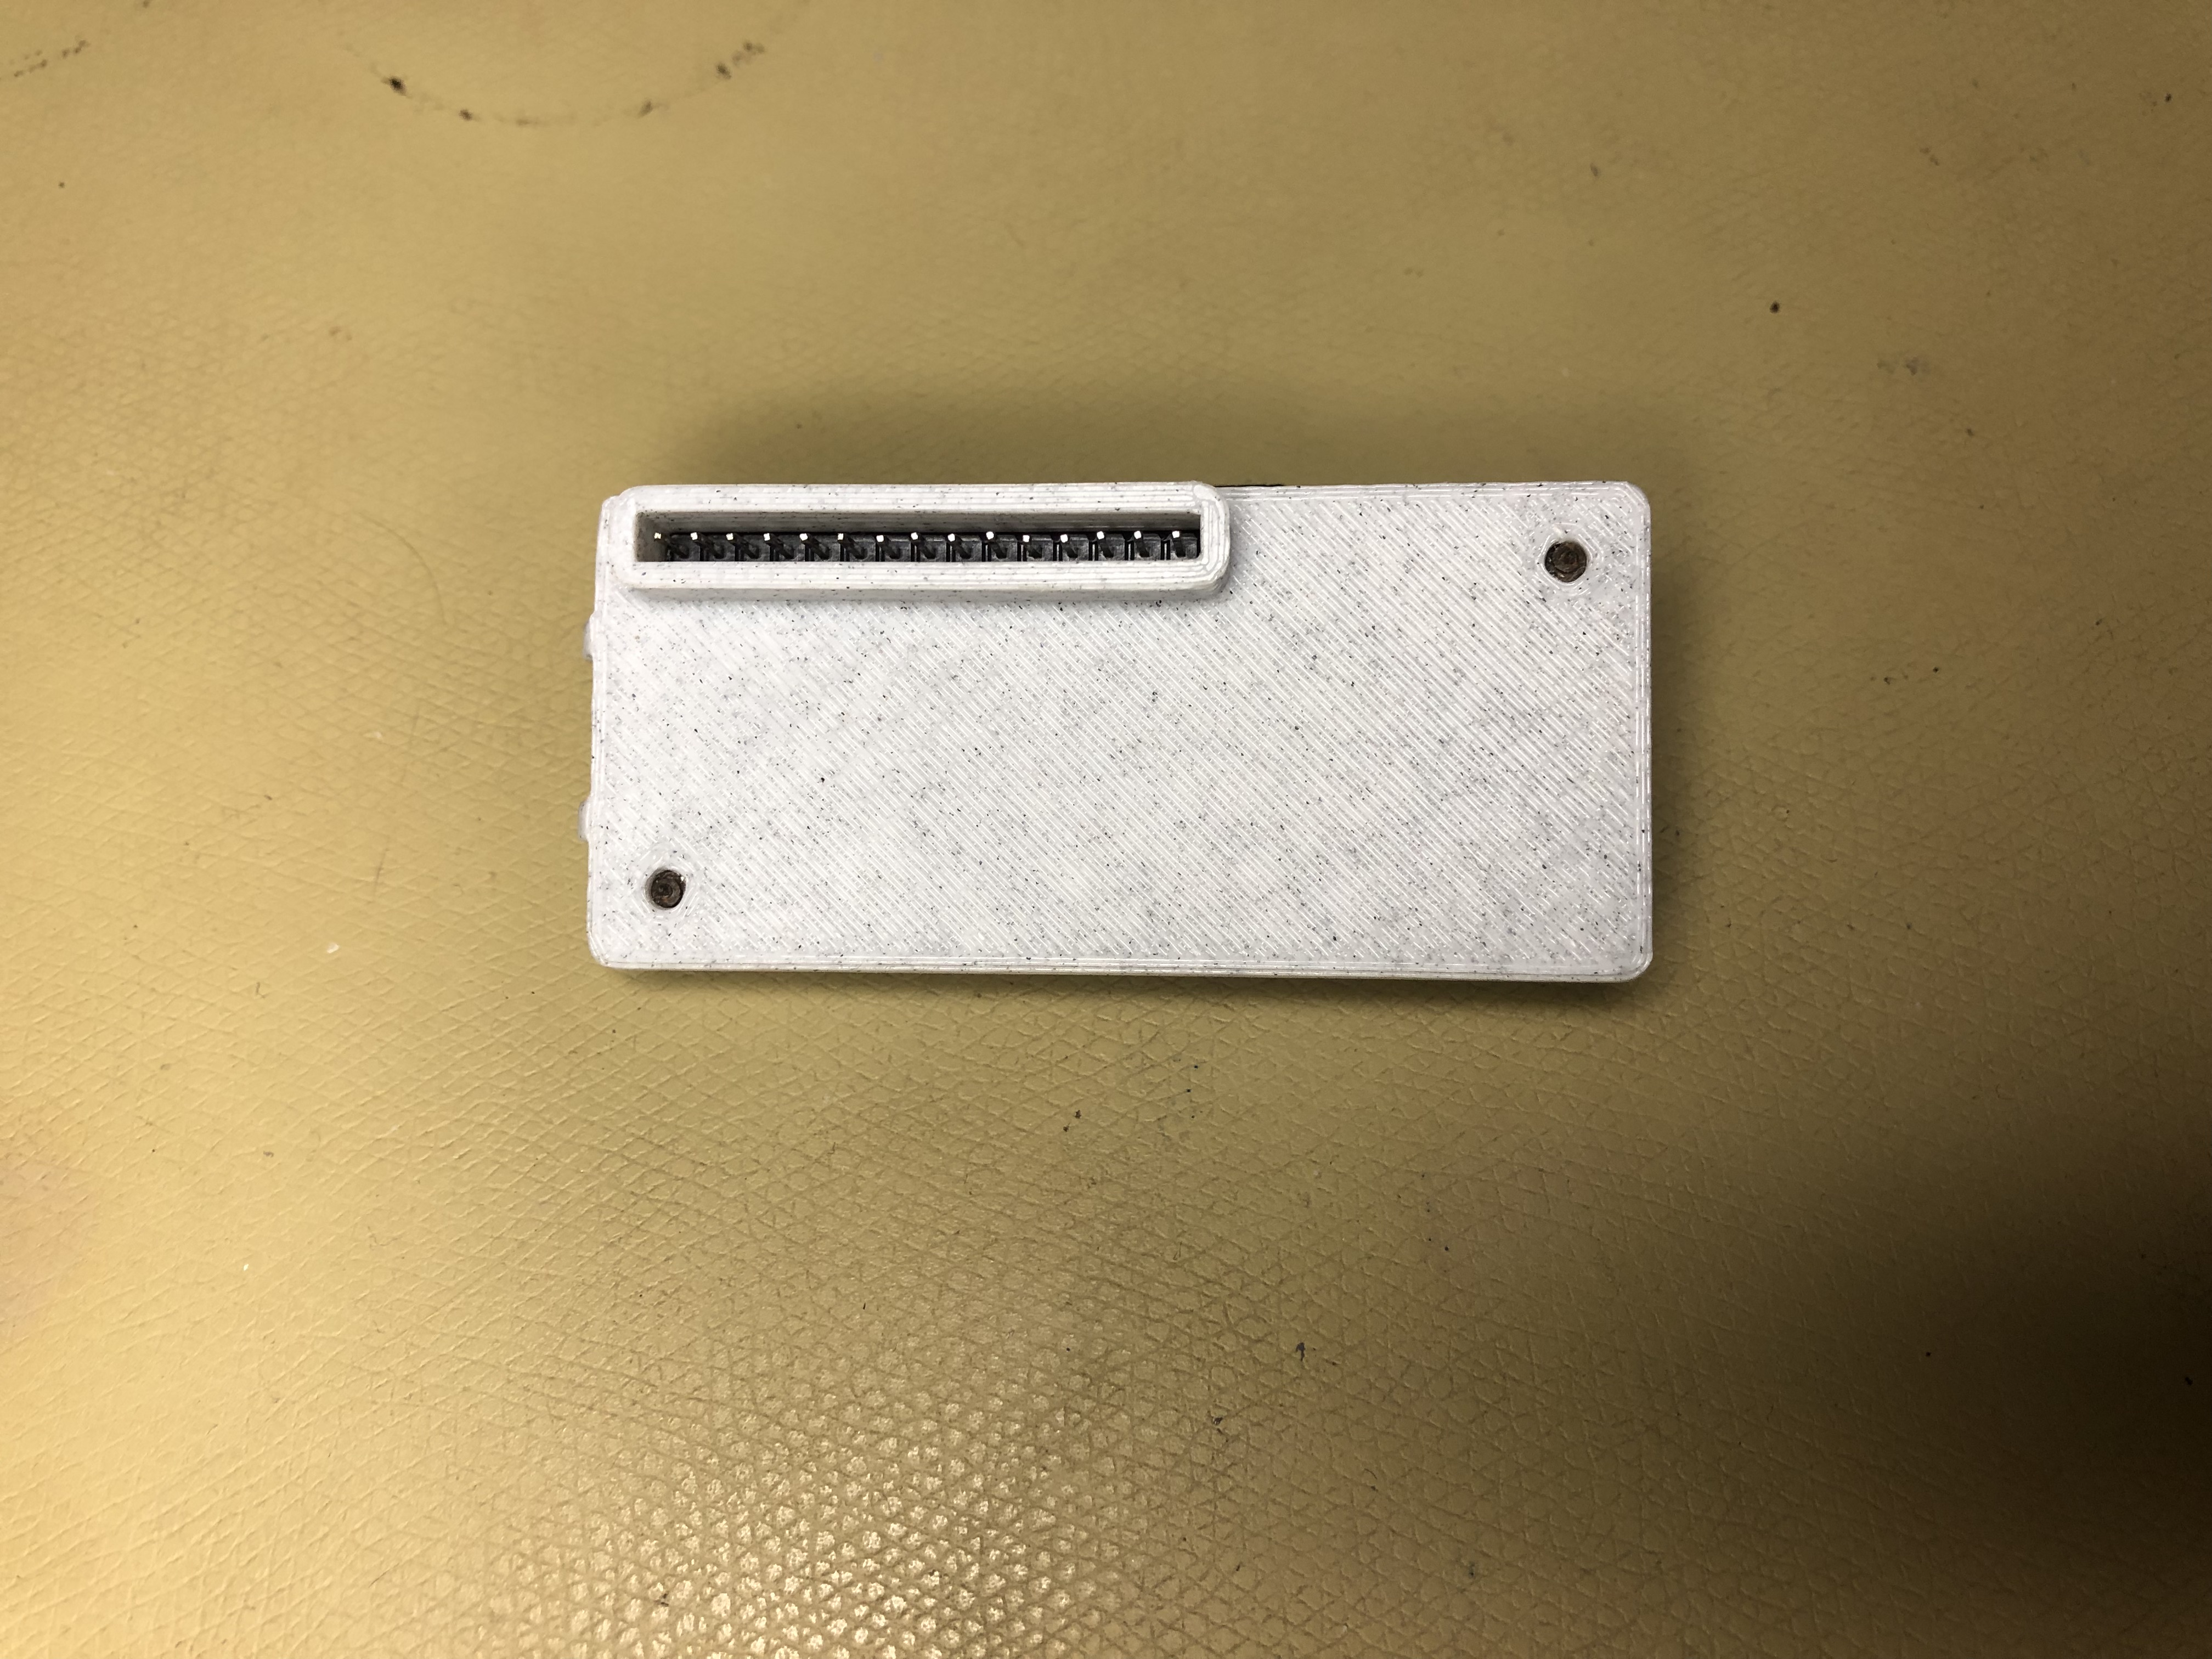
\includegraphics[width=0.8\textwidth]{assets/case/Node-Bot.JPG}
            \caption{Bottom view.}
        \end{figure}

    \FloatBarrier \newpage
    \subsection{Battery}

        \begin{figure}[H]
            \centering
            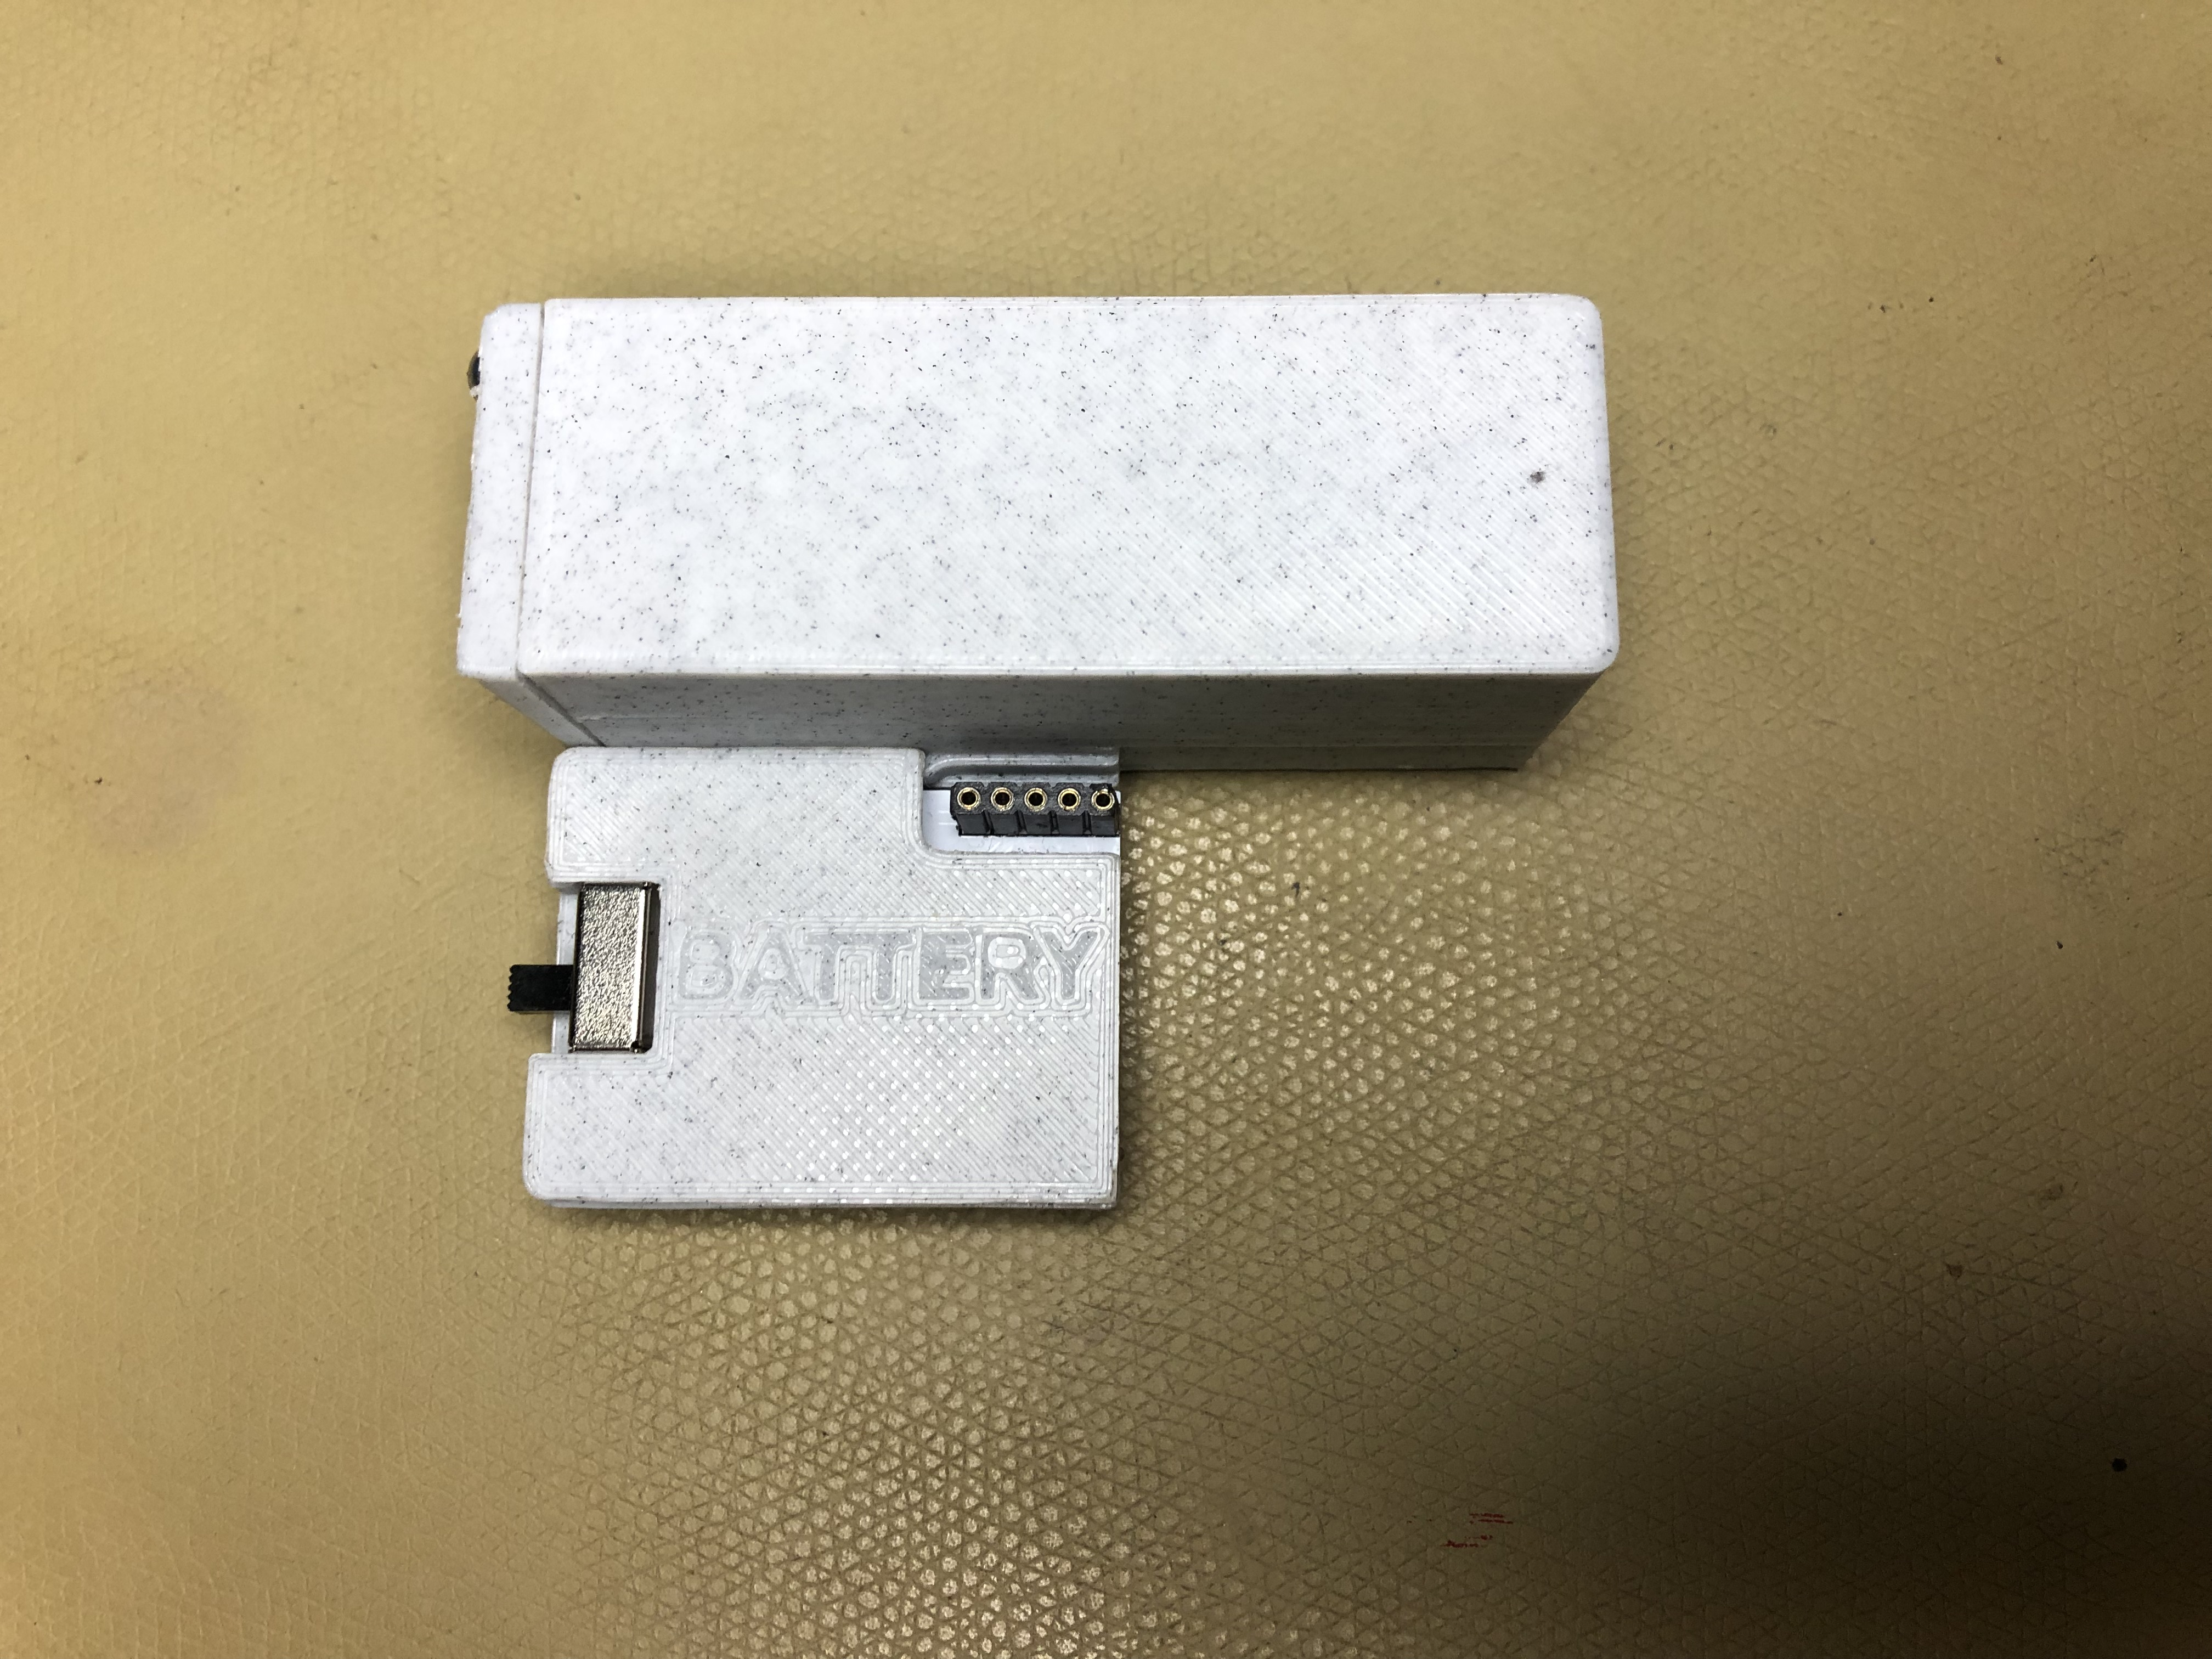
\includegraphics[width=0.8\textwidth]{assets/case/Battery-Top.JPG}
            \caption{Top view.}
        \end{figure}

        \begin{figure}[htbp]
            \centering
            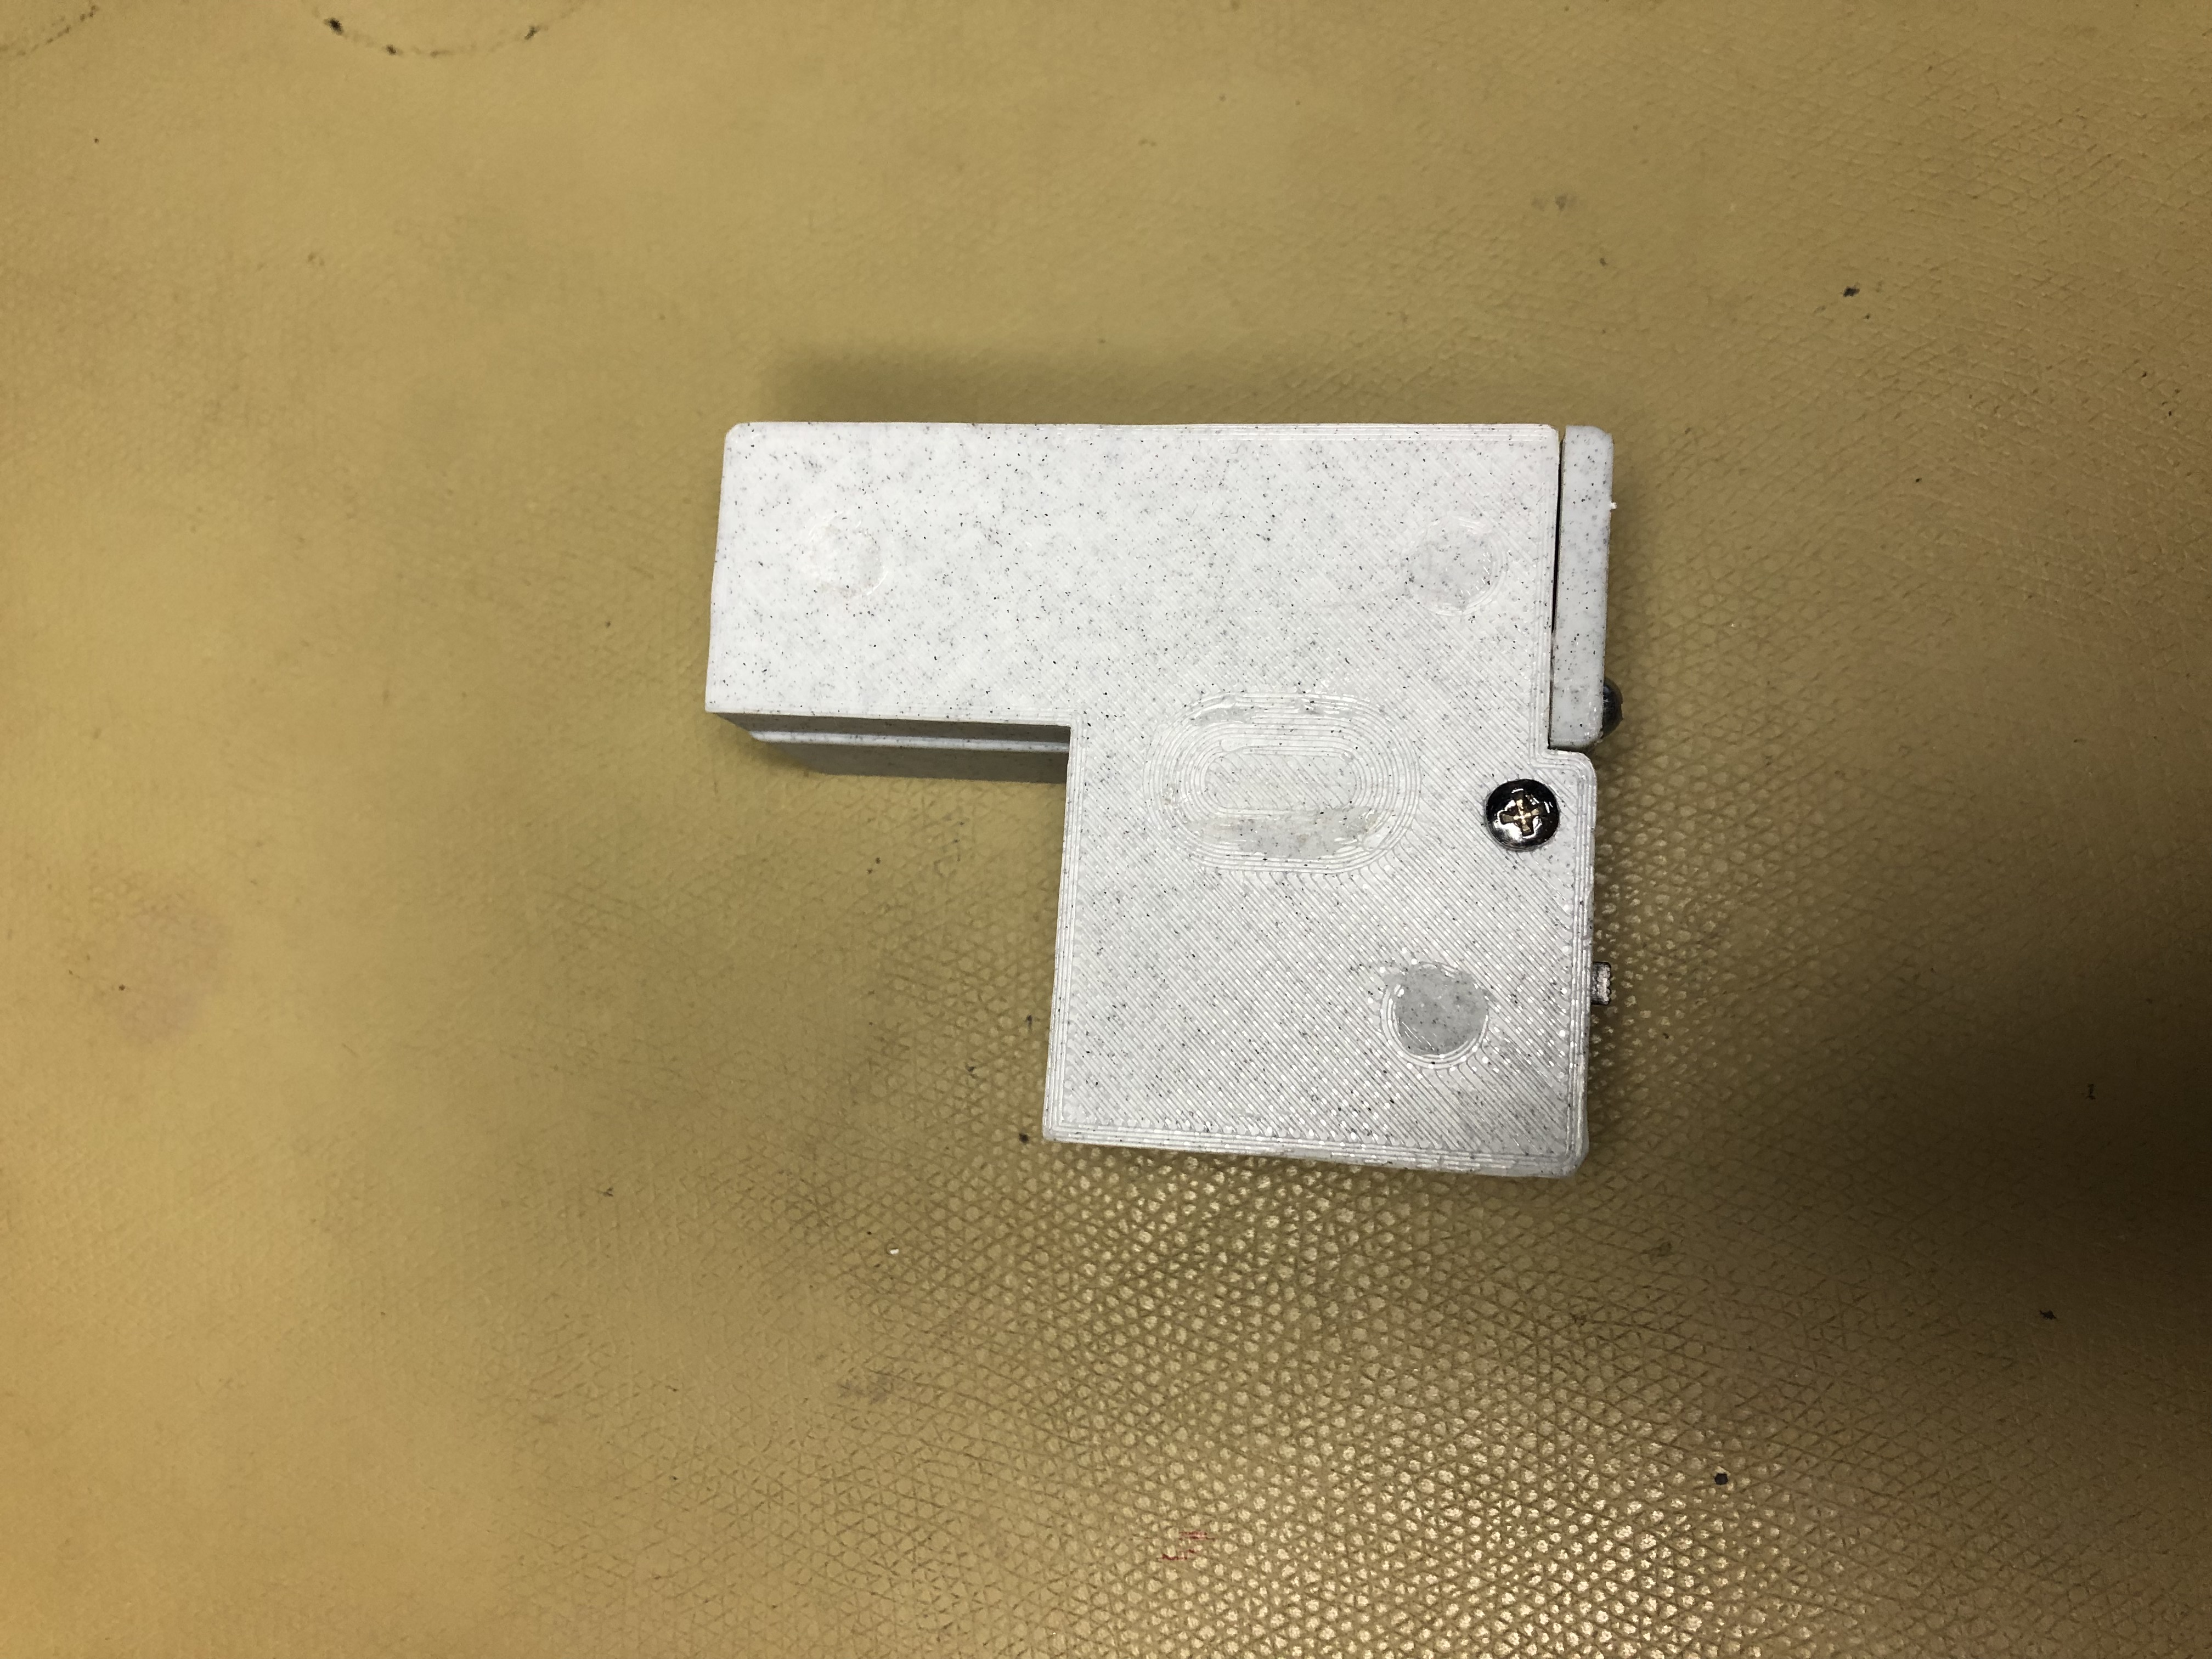
\includegraphics[width=0.8\textwidth]{assets/case/Battery-Bot.JPG}
            \caption{Bottom view.}
        \end{figure}

        \begin{figure}[htbp]
            \centering
            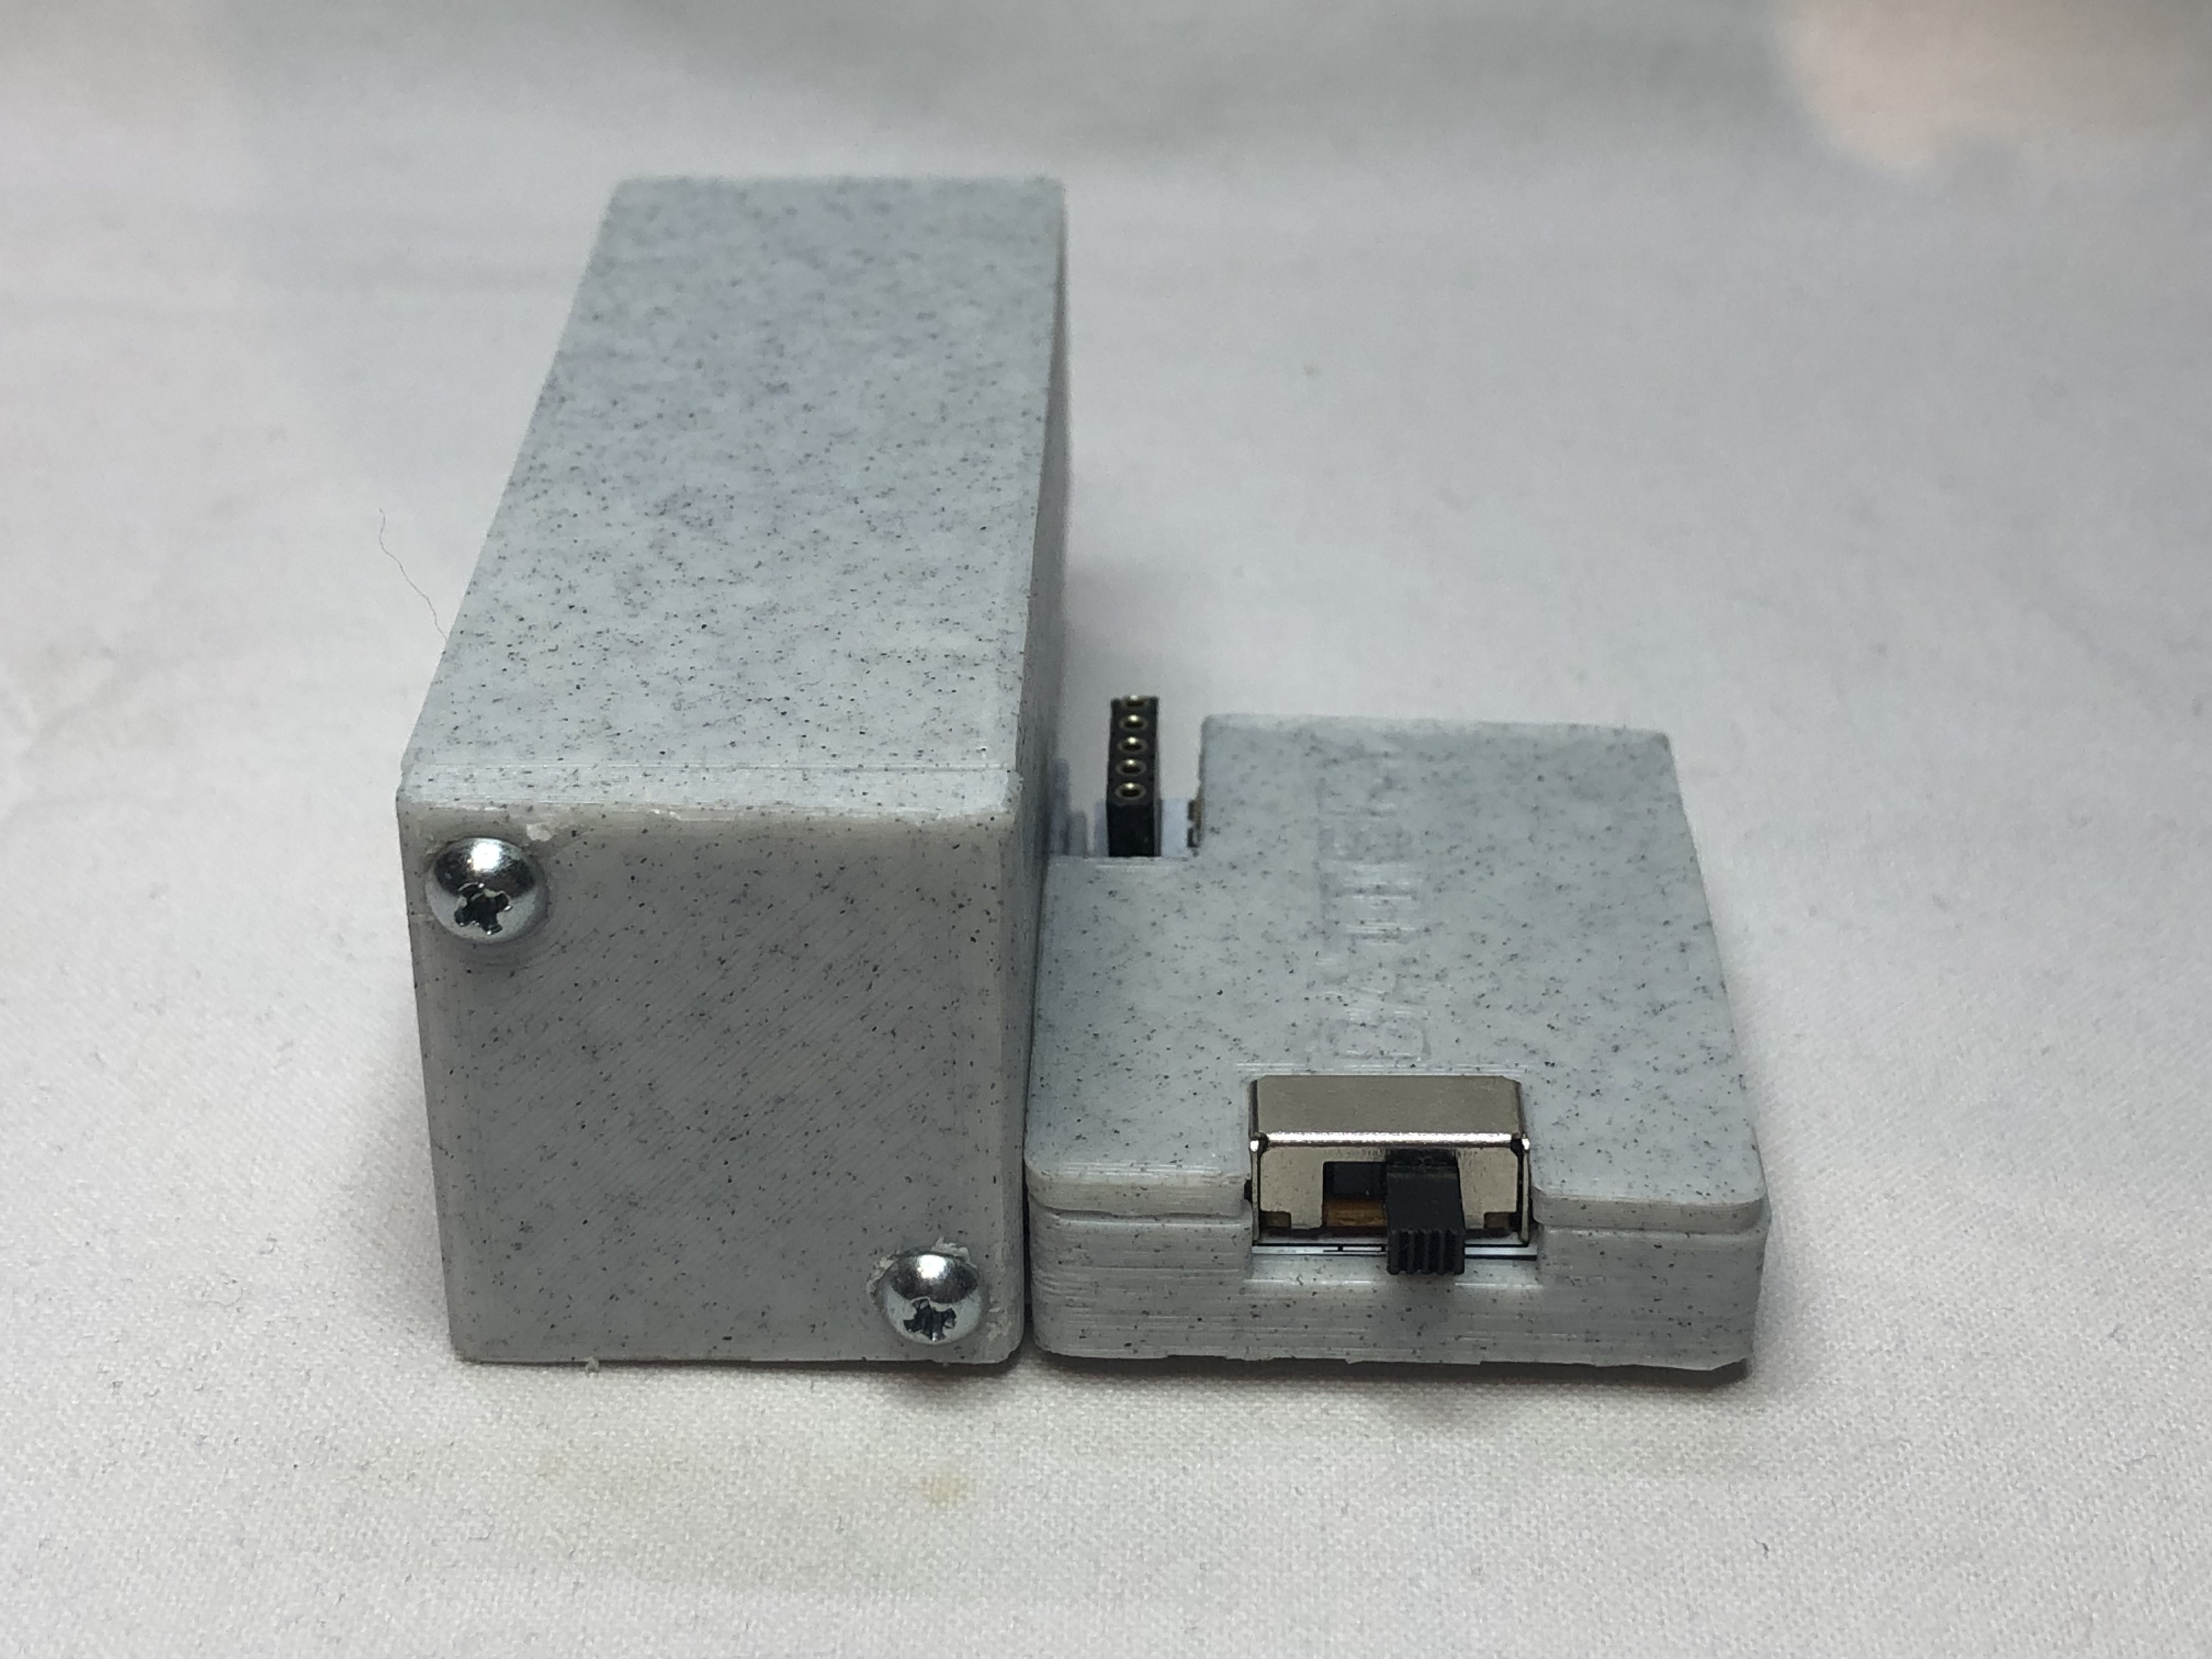
\includegraphics[width=0.8\textwidth]{assets/case/Battery-Side.JPG}
            \caption{Side view.}
        \end{figure}

    \FloatBarrier
    \subsection{Motion}

        This case consists of two parts, the top and the bottom. 
        \begin{figure}[htbp]
            \centering
            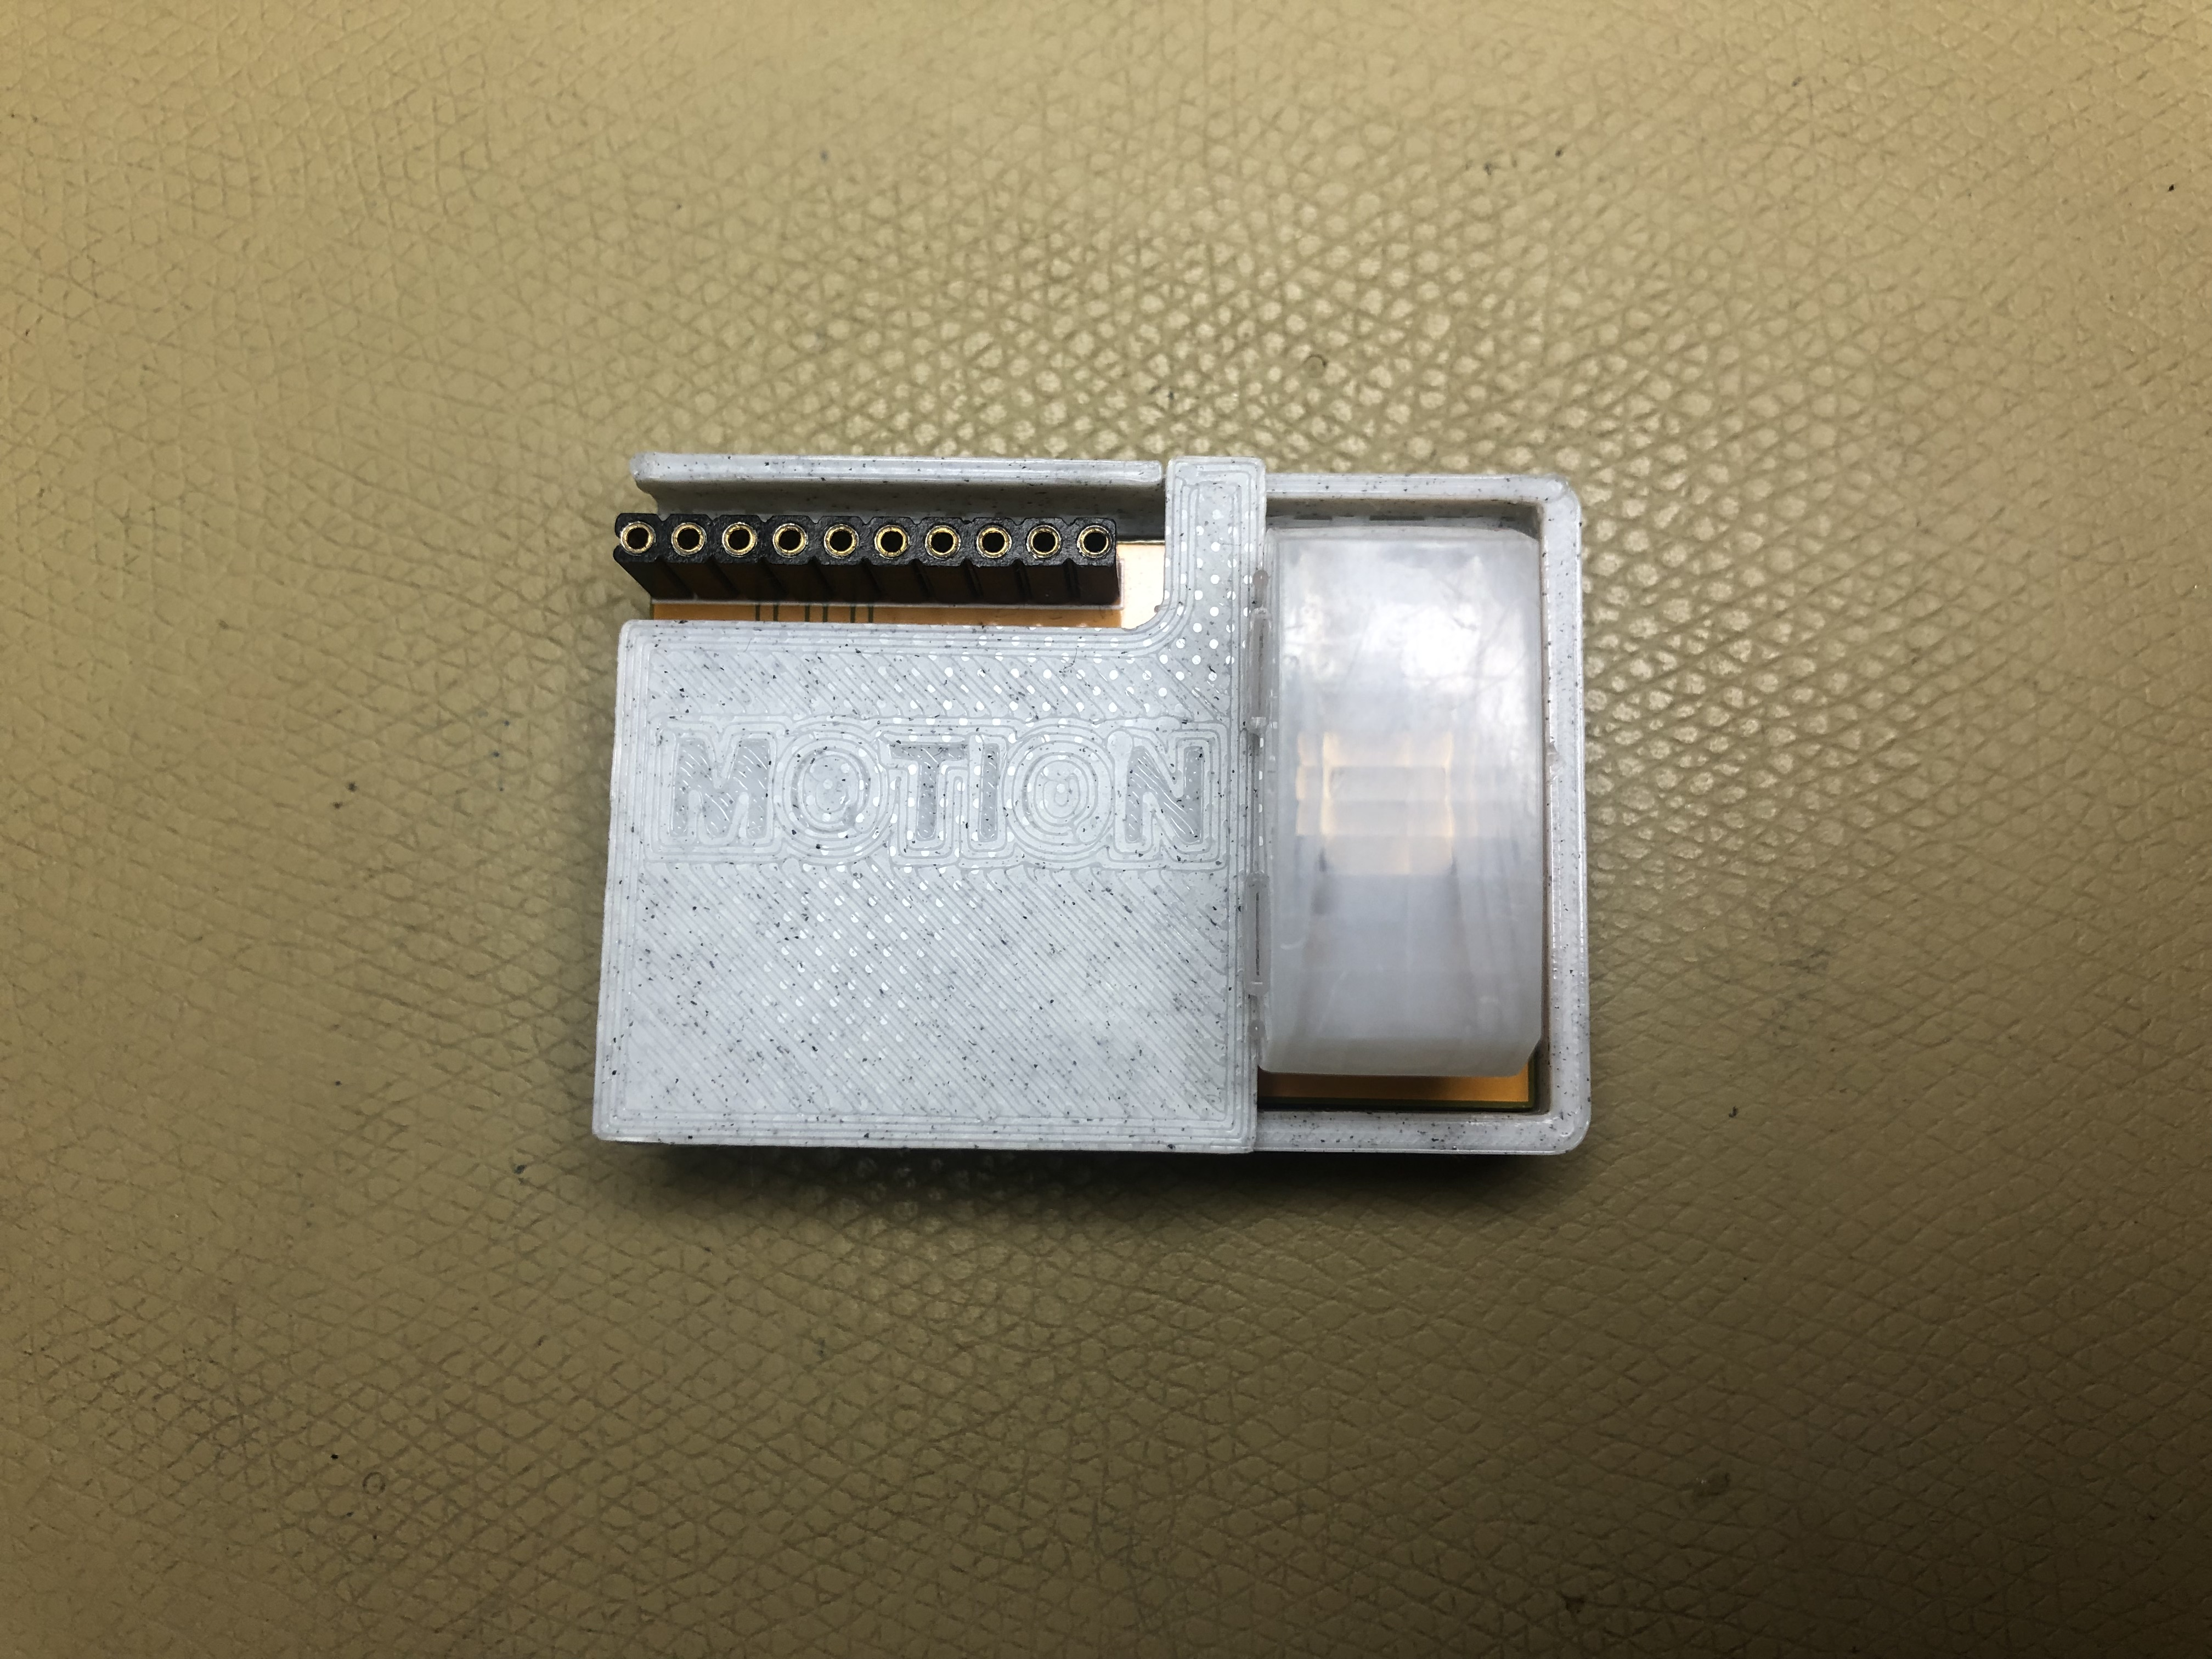
\includegraphics[width=0.8\textwidth]{assets/case/Motion-Top.JPG}
            \caption{Top view.}
        \end{figure}
        
        \begin{figure}[htbp]
            \centering
            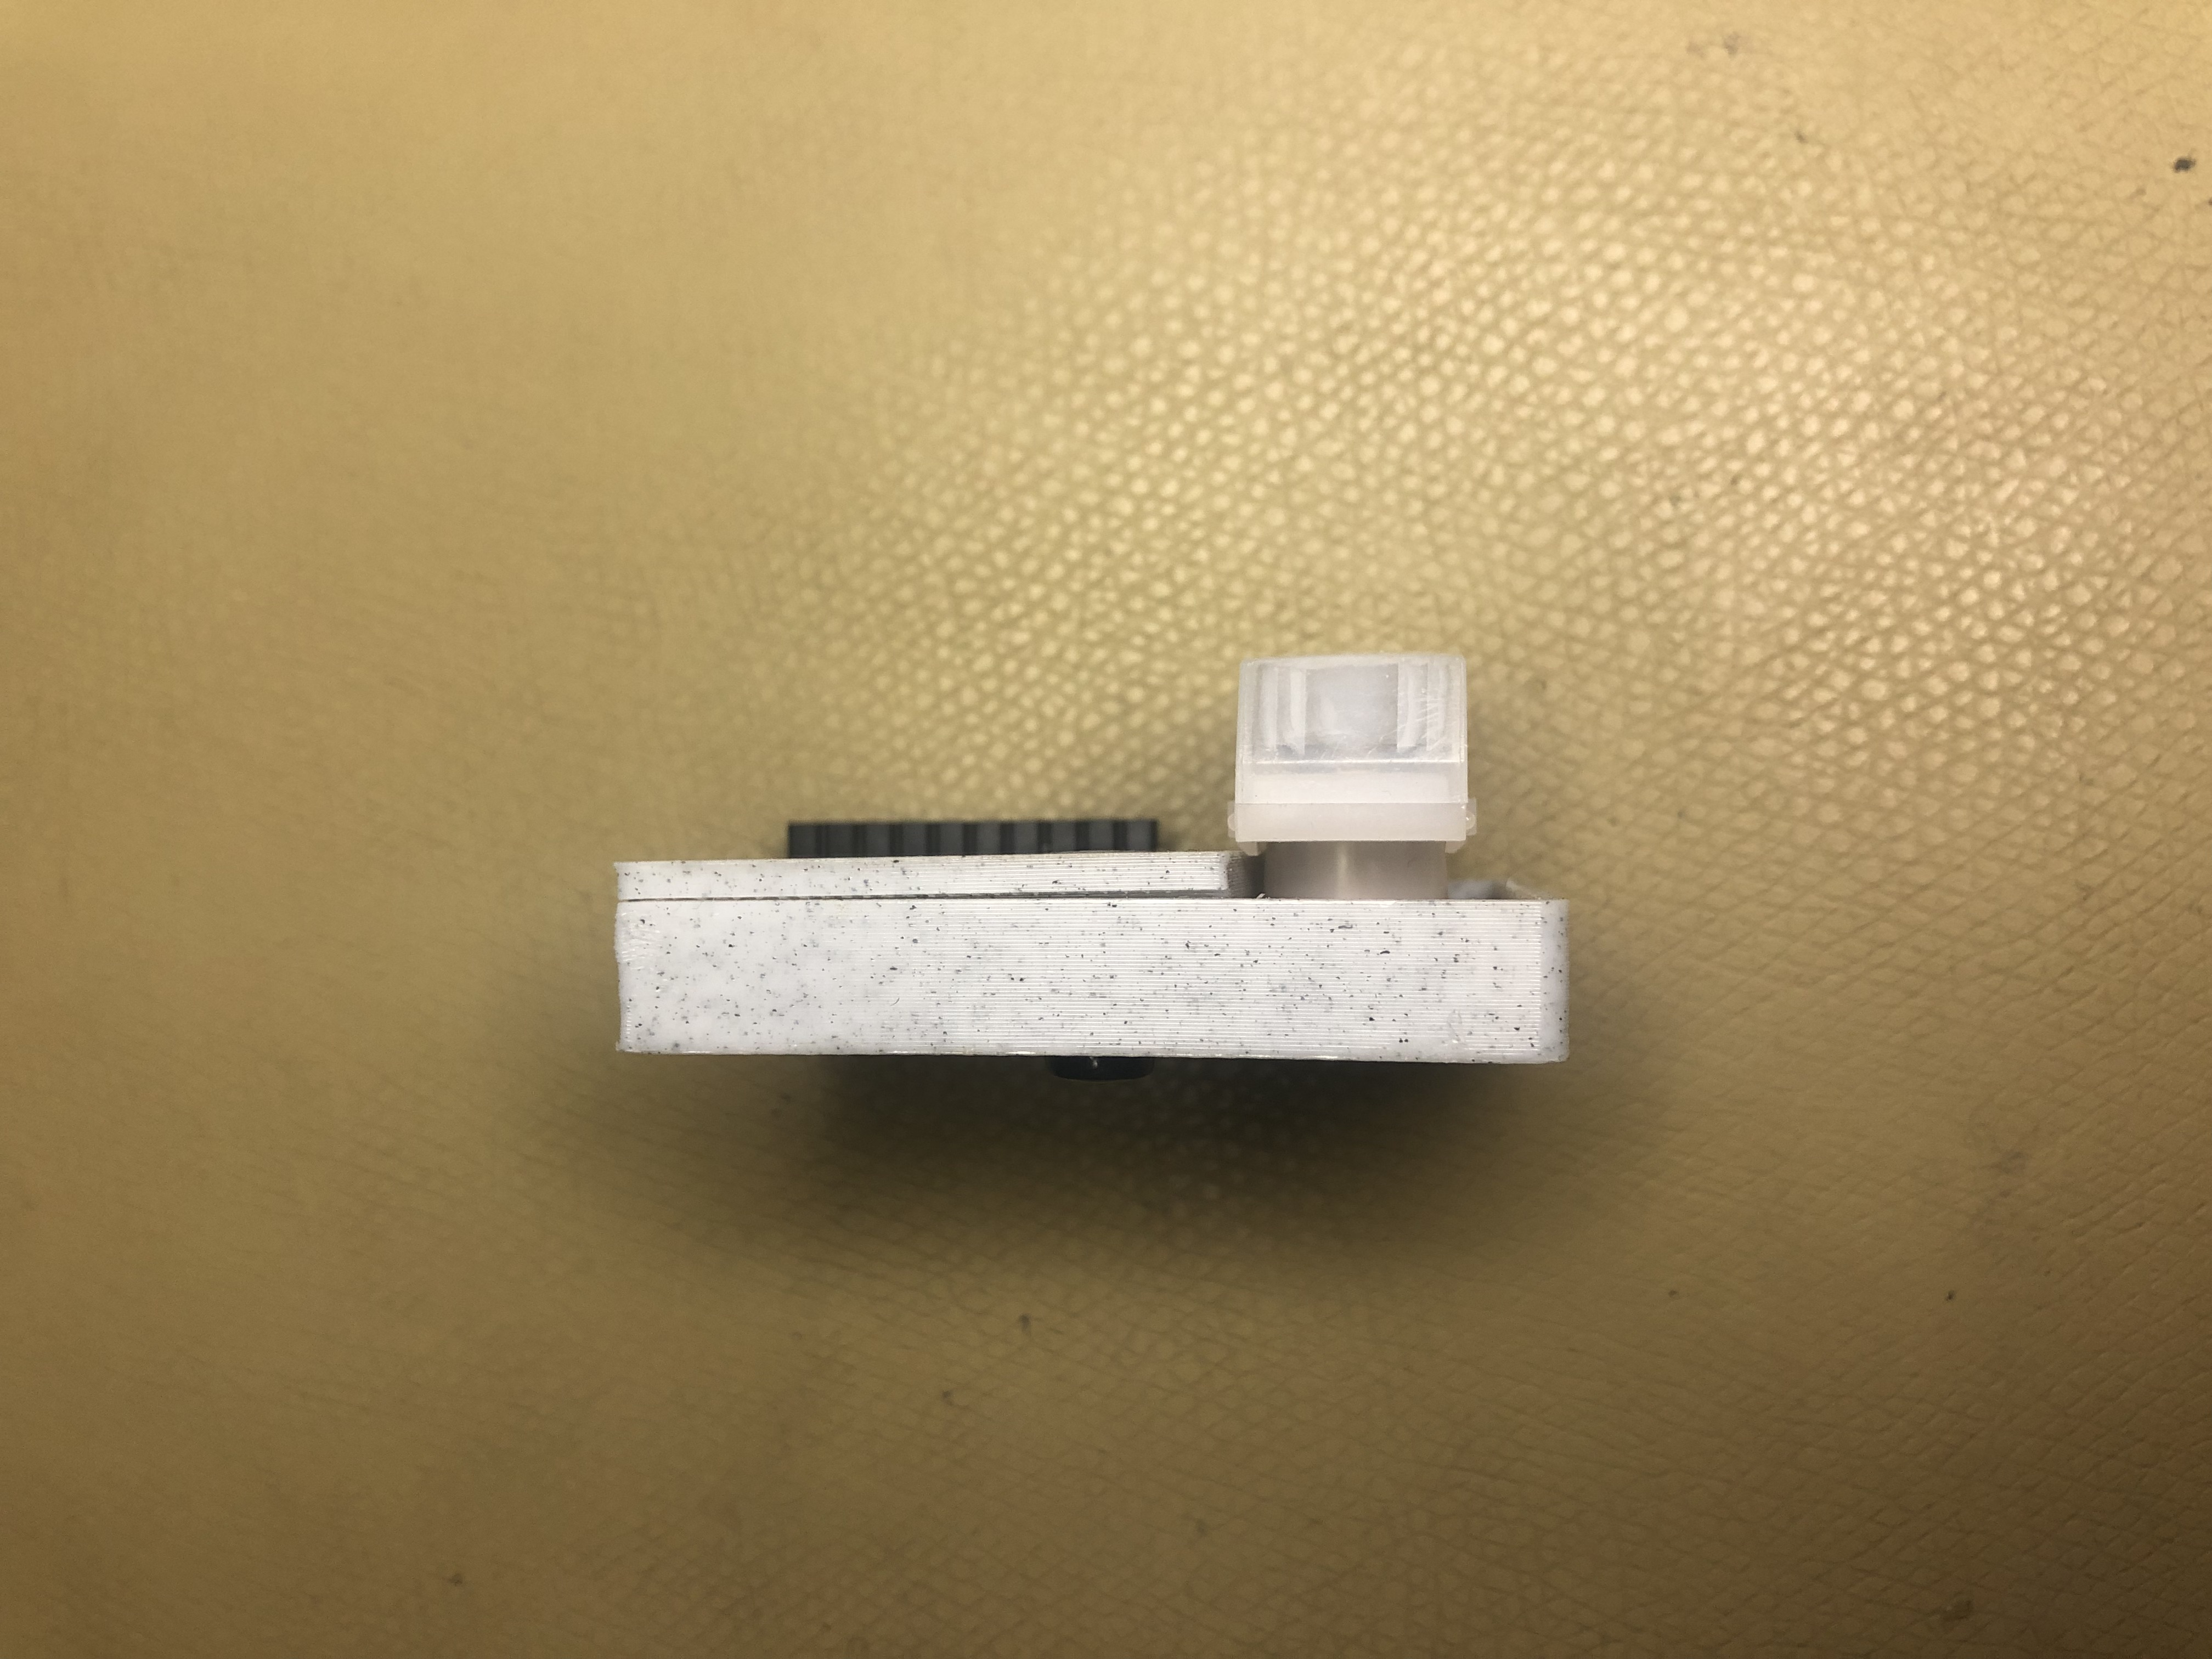
\includegraphics[width=0.8\textwidth]{assets/case/Motion-Side.JPG}
            \caption{Side view.}
        \end{figure}
        

        \FloatBarrier 
    \subsection{Switch}
            
            \begin{figure}[H]
                \centering
                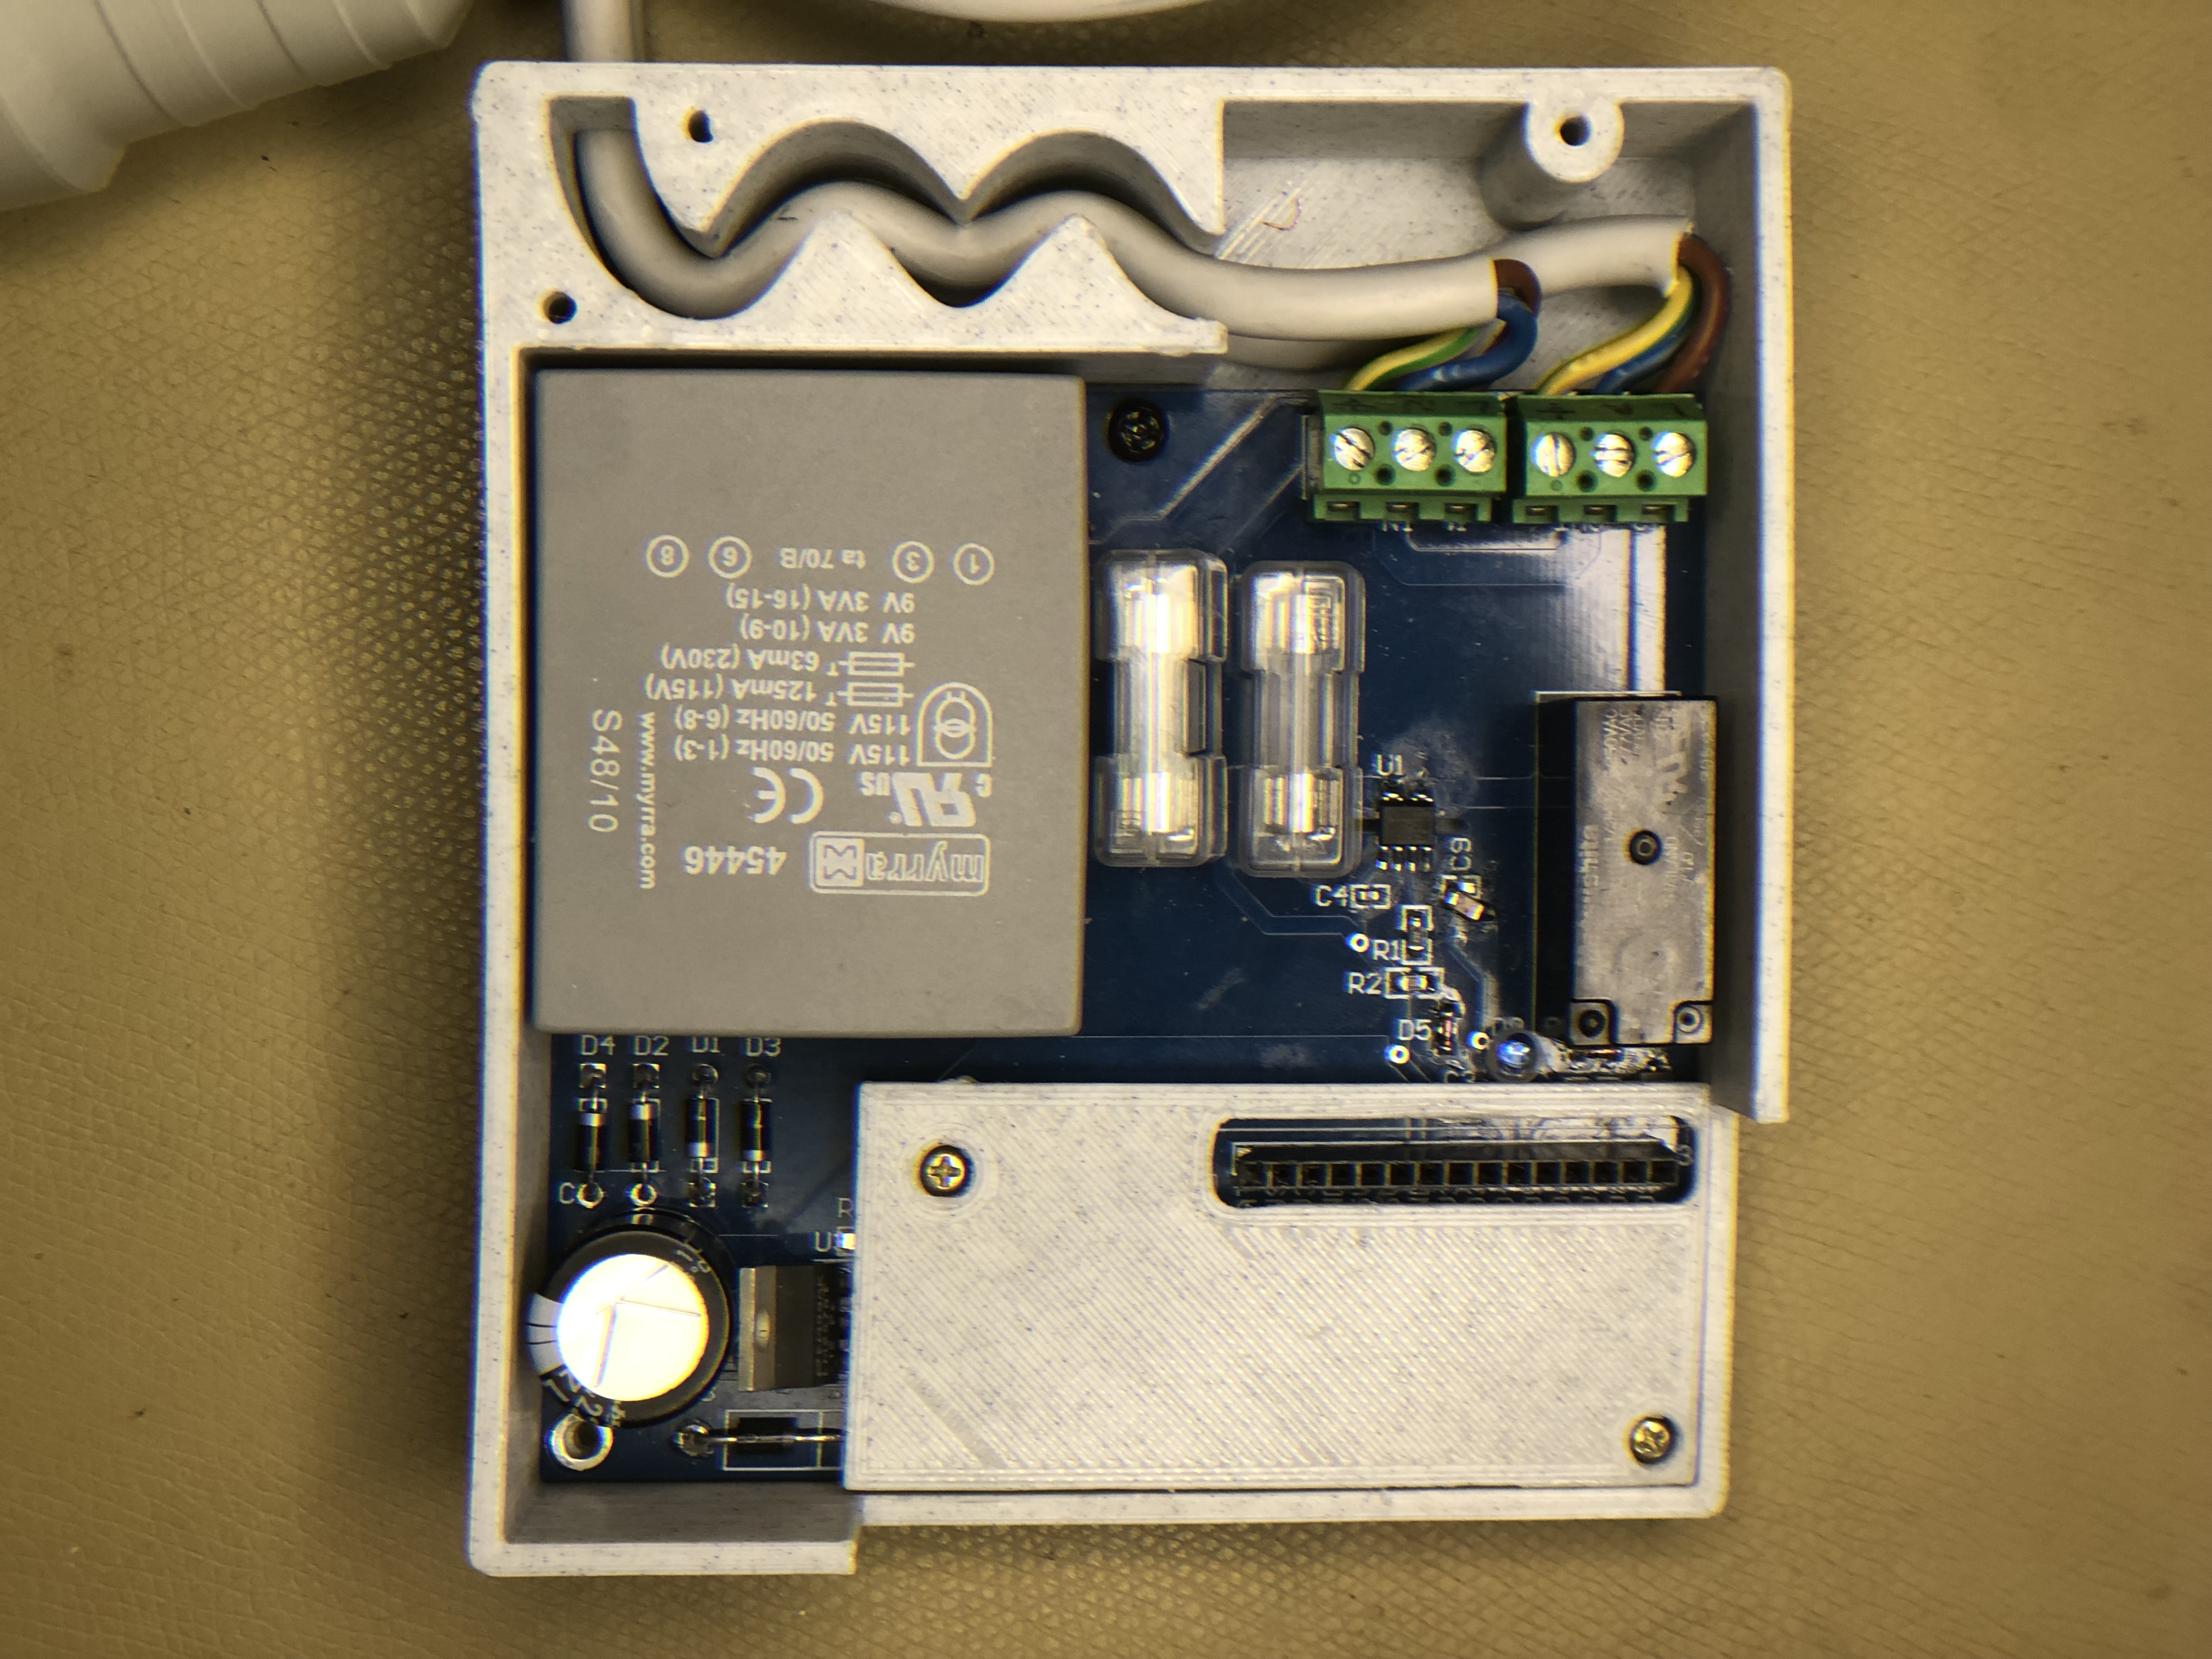
\includegraphics[width=0.8\textwidth, angle = 0]{assets/case/Switch-Open1.JPG}
                \caption{Case open top view.}
            \end{figure}
    
            \begin{figure}[htbp]
                \centering
                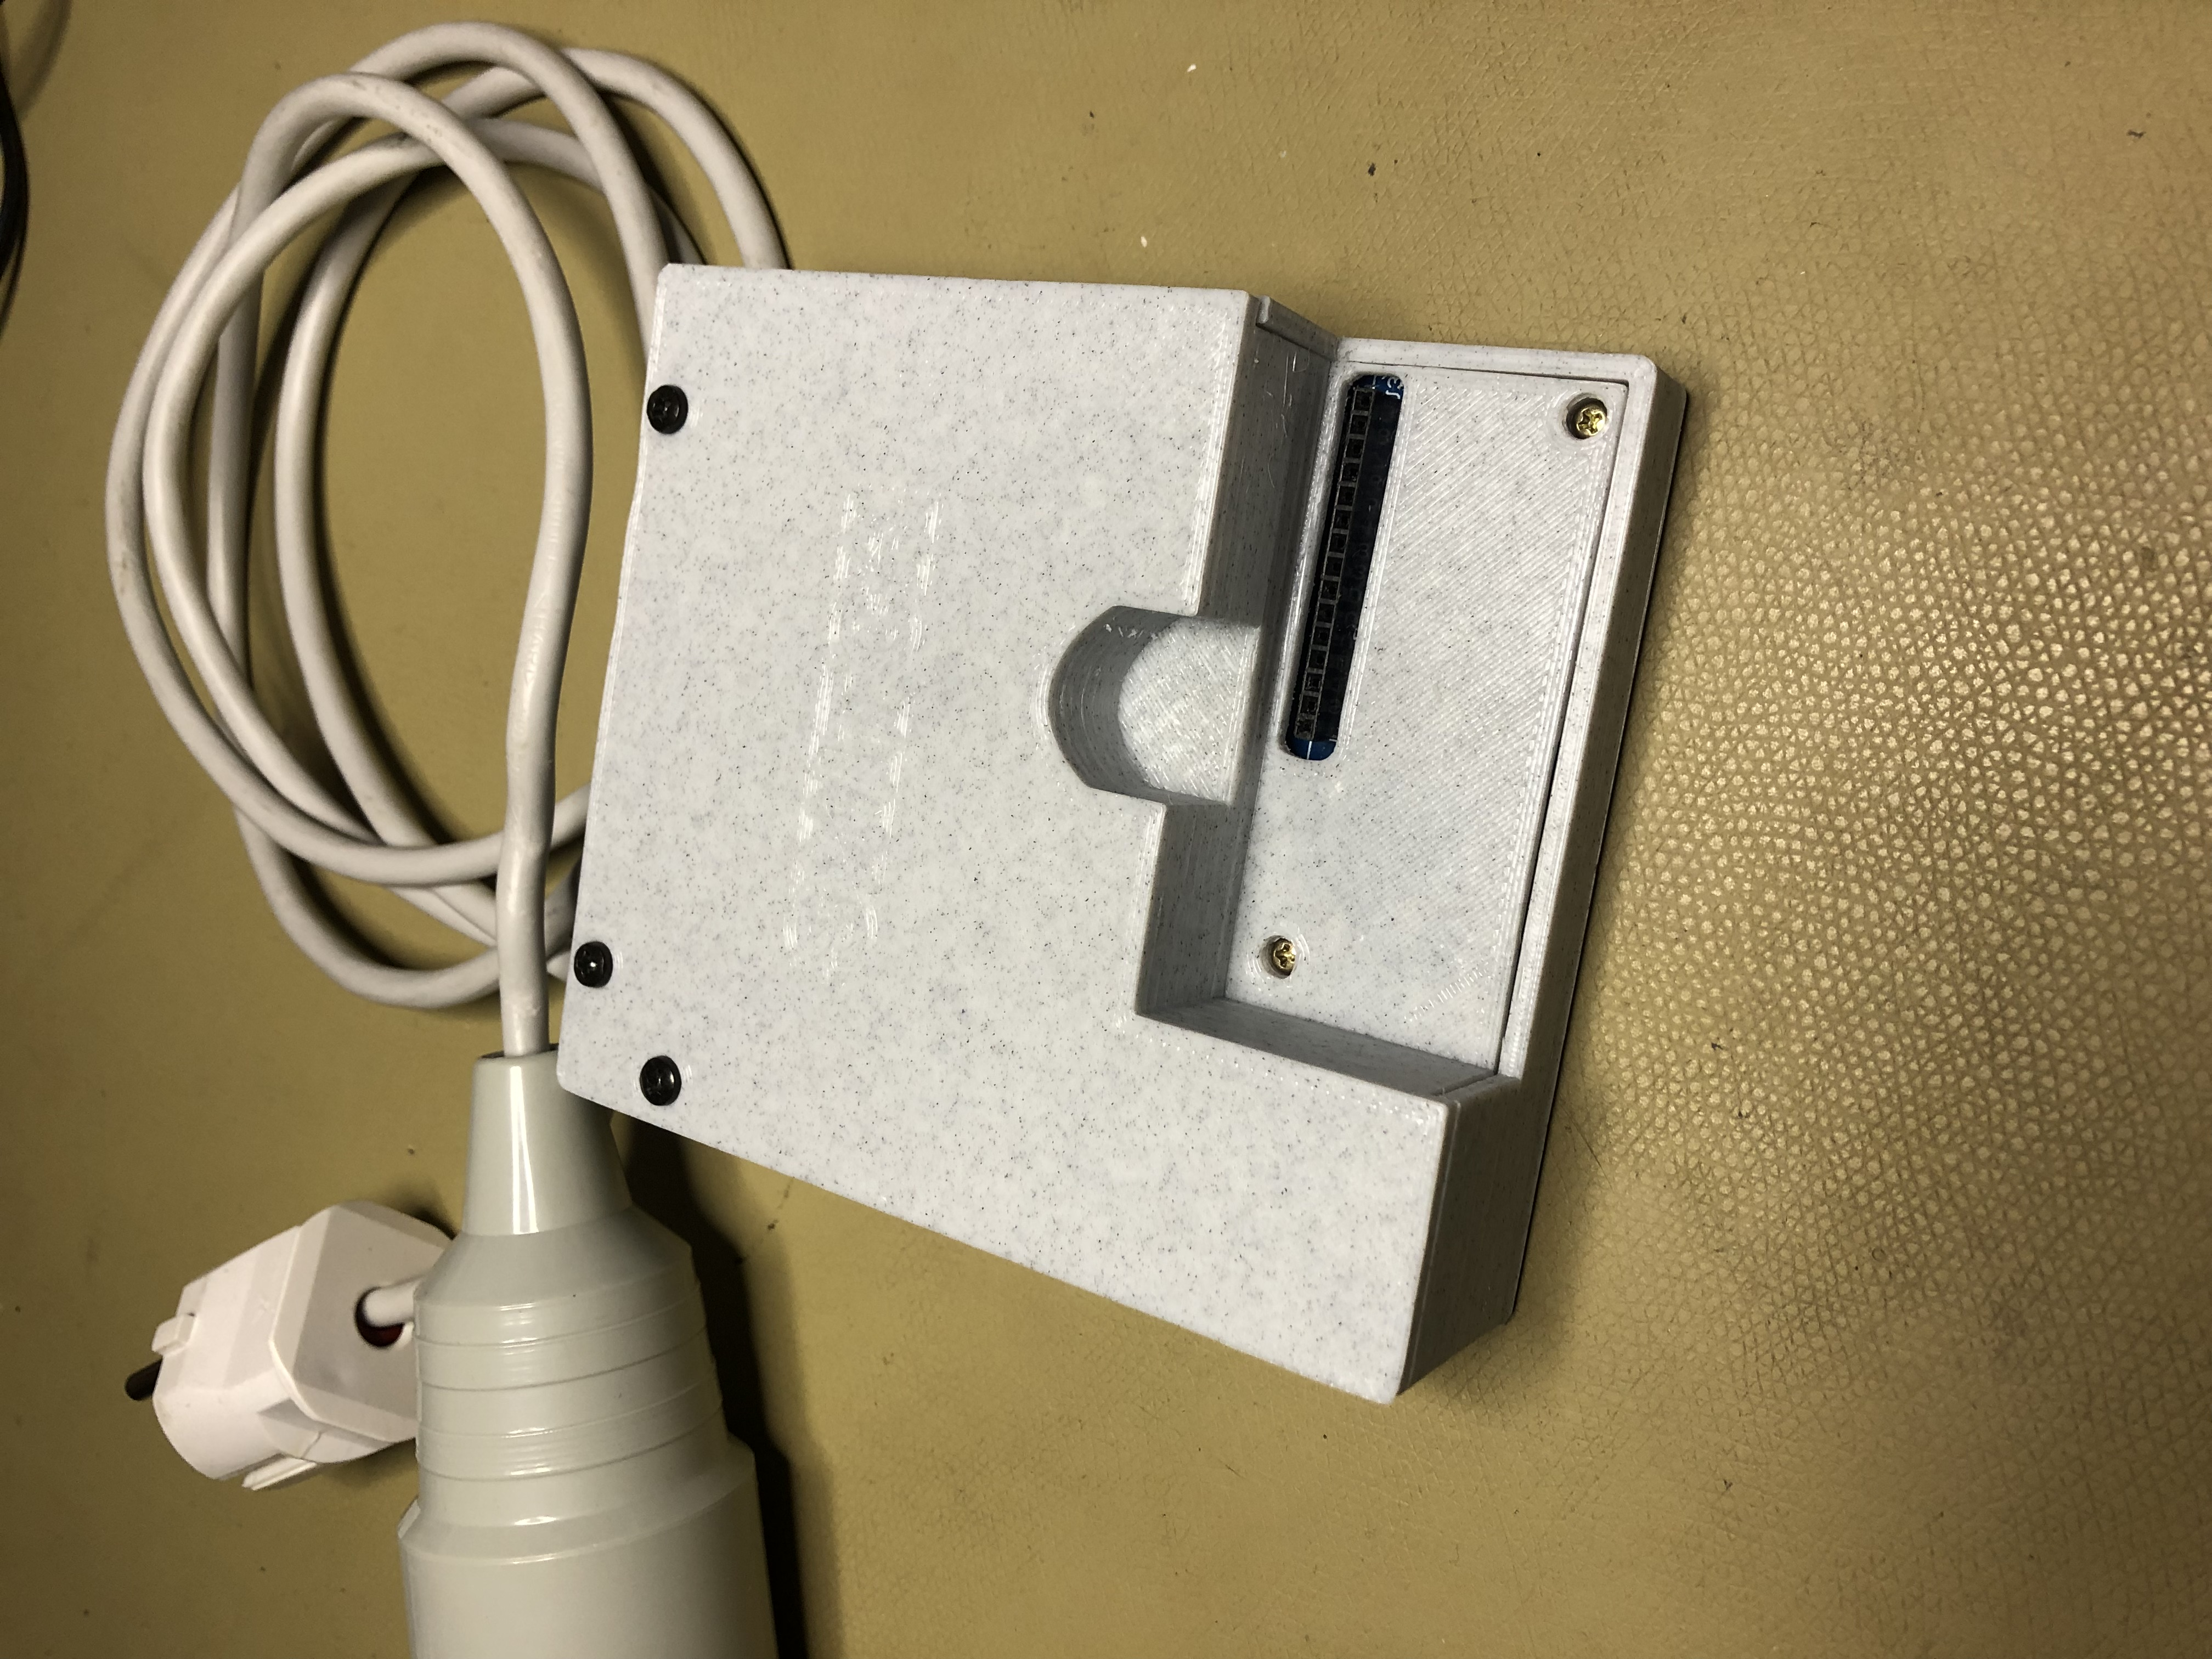
\includegraphics[width=0.8\textwidth, angle = -90]{assets/case/Switch-Closed2.JPG}
                \caption{Case closed top view.}
            \end{figure}
            
    \FloatBarrier
    \subsection{Combined Module}
    
        
        